\chapter{Feynman Diagrams}

In the previous chapters we have seen how to calculate Green's functions in QFT and, as we have notice, the number of terms in the expansion of the Green's function grows very quickly as we increase the order of the correction, making it very difficult to keep track of all the terms and their contributions. This is where Feynman diagrams come in handy, as they provide a \textbf{visual representation of the interactions} and allow us to easily keep track of the different terms in the expansion.

In this chapter we will see how to derive a set of practical rules, known as Feynman rules, that allow us to compute Green's functions and scattering amplitudes in a systematic way for an \textit{interacting theory in perturbation theory}, without having to calculate all the contractions explicitly. This method is based on Tylor expansions in the coupling constants \(g_j\), assuming a weak enough interaction, and it is a very powerful tool for calculating physical quantities in QFT, as it allows us to write down the contribution of each diagram without having to calculate all the contractions explicitly, which is a very powerful tool for calculating physical quantities in QFT.

We will start by reviewing the Hamiltonian formalism and the interaction picture, which are essential for understanding how to calculate Green's functions in an interacting theory, and then we will see how to derive the Feynman rules for a simple interacting theory, and how to use them to calculate physical quantities. Through some examples, we will see how to apply the Feynman rules in practice, and then we will see how to generalize them to more complicated theories and to momentum space, which is the most common way to use Feynman diagrams in QFT.

\section{Hamiltonian Formalism and Interaction Picture}

In QFT is often more convenient to work in the Hamiltonian formalism, where we express the dynamics of the system in terms of a Hamiltonian operator. The Hamiltonian can be split into a free part, which describes non-interacting particles, and an interaction part, which describes the interactions between particles.

The \textbf{Heisenberg picture} is often used in QFT, where operators evolve in time while states remain constant. However, for perturbative calculations, it is more convenient to use the \textbf{interaction picture}, where both operators and states evolve in time. Let us start from the Heisenberg equation of motion for an operator \( \hat{O}(x) \):
\[
    i \partial_t \hat{O}(x) = [\hat{O}(x), \hat{H}(x)],
\]
where \(\hat{H}(x)\) is the Hamiltonian operator. We can write the solution to this equation through the time evolution operator \(\hat{S}(t, t_0)\) as
\[
    \hat{O}(\mathbf{x}, t) = \hat{S}^{\dagger}(t, t_0) \hat{O}(\mathbf{x}, t_0) \hat{S}(t, t_0),
\]
which can be inserted back into the Heisenberg equation of motion to get an equation for the time evolution operator:
\[
    i \partial_t \hat{S}(t, t_0) = \hat{H}(t) \hat{S}(t, t_0).
\]

Now let us split the Hamiltonian into a free part and an interaction part:
\[
    \hat{H}(t) = \hat{H}_0 + \hat{V}(t),
\]
and the Lagrangian into a free part and an interaction part:
\[
    \mathcal{L} = \mathcal{L}_0 + \mathcal{L}_{\text{int}}.
\]
In practice, \(\hat{H}_0\) will be the Hamiltonian of a free theory, which describes non-interacting particles whose dynamics can be solved exactly, while \(\hat{V}(t)\) will be the interaction Hamiltonian, which will be treated as a perturbation and encodes all the interaction terms. The free part of the Lagrangian \(\mathcal{L}_0\) will describe the dynamics of the free fields, while the interaction part \(\mathcal{L}_{\text{int}}\) will describe the interactions between the fields, indeed we can write the Legendre transform of the Lagrangian to get the Hamiltonian as
\[
    H = \int \mathrm{d}^3 \mathbf{x} \, \mathcal{H} (\mathbf{x}), \quad \begin{dcases}
        \mathcal{H} = \pi \dot{\phi} - \mathcal{L}, \\
        \pi = \partial \mathcal{L} / \partial \dot{\phi},
    \end{dcases}
\]
and if \(\mathcal{L}_{\text{int}} \) does not contain derivatives, then we simply have \(\mathcal{H}_{\text{int}} = - \mathcal{L}_{\text{int}} \), and thus we can write the interaction Hamiltonian as
\[
    V = - \int \mathrm{d}^3 \mathbf{x} \, \mathcal{L}_{\text{int}}.
\]
If \(\mathcal{L}_{\text{int}} \) does indeed contain derivatives, then similar results can be obtained, but it will be easier to derive them in the Lagrangian formalism, which is more convenient for theories with derivative interactions, and we will see how to do that in the next chapters.

\subsection{Interaction Picture}

We are now moving from the Heisenberg picture to the interaction picture, where both operators and states evolve in time. In the interaction picture, the \textit{fields evolve according to the free Hamiltonian} \(H_0\), while the \textit{states evolve according to the total Hamiltonian} \(V\): the interaction is encoded in the evolution of the states, while the fields evolve as if they were free fields. This is a very important point, as it allows us to use the free fields to calculate the interactions, which is much easier than dealing with the full interacting fields.

Then of course the \textit{matrix elements} we are interested in computing \textit{will be independent from the chosen picture}, since they are physical quantities, and thus we can choose the picture that is more convenient for our calculations. Schrödinger, Heisenberg and interaction picture are just different ways of describing the same physics, and they are identically equivalent equivalent at a conventional reference time \(t = t_0\).

Thus we can start from the Schrödinger picture, where the fields are time-independent, and then we can move to the interaction and Heisenberg picture, where the fields evolve in time according to the free Hamiltonian and the total Hamiltonian respectively. We can write the fields in the different pictures and see how they are related to each other as
\[
    \begin{dcases}
        \hat{\phi}_0 = \hat{\phi}_I = e^{i \hat{H}_0 (t-t_0)} \hat{\phi}_S e^{-i \hat{H}_0 (t-t_0)}, \quad \hat{\phi}_S = \hat{\phi}_I (t=t_0) \\
        \hat{\phi} = \hat{\phi}_H = \hat{S}^{\dagger}(t,t_0) \hat{\phi}_S \hat{S}(t,t_0) = \hat{U}^{\dagger} (t,t_0) \hat{\phi}_I \hat{U}(t,t_0),
    \end{dcases}
\]
where
\[
    \hat{U}(t,t_0) = e^{i \hat{H}_0 (t-t_0)} \hat{S}(t,t_0),
\]
is the time evolution operator connecting the interaction picture to the Heisenberg picture, while \(\hat{S}(t,t_0)\) is the time evolution operator connecting the Schrödinger picture to the Heisenberg picture.

Now having \(\hat{H}_H = \hat{H}_S\) and \(\hat{H}_0 = \hat{H}_{0,S}\) (i.e. the Heisenberg Hamiltonian is the same as the Schrödinger Hamiltonian, and the free Hamiltonian is the same in both pictures) we can write the equation of motion for \(\hat{U}\) by inserting the fields in the Heisenberg equation of motion, which gives
\[
    i \partial_t \hat{U}(t,t_0) = \hat{V}_I (t,t_0) \hat{U}(t,t_0),
\]
with
\[
    \hat{V}_I = e^{i \hat{H}_0 (t-t_0)} \hat{V}_S e^{-i \hat{H}_0 (t-t_0)},
\]
which is the \textbf{interaction potential} (potential in the interaction picture). In practice, since \(\hat{V}\) is given by the integral of the interaction Lagrangian, we can write it as
\[
    \hat{V}_I = \hat{V}_S(\hat{\phi}) \big|_{\hat{\phi} \to \hat{\phi}_I} = \hat{V}(\hat{\phi}_0),
\]
which means that the potential in the interaction picture is the same as the potential in the Schrödinger picture, but with the fields replaced by their interaction picture counterparts (which is the same as the free fields). This is a very important result, as it allows us to use the free fields to calculate the interactions, which is much easier than dealing with the full interacting fields.

\subsubsection{Dyson Series}

The solution to the evolution equation for \(\hat{U}\) can be written as the following well-known time-ordered exponential:
\[
    \hat{U}(t,t_0) = \hat{T} \exp \left( -i \int_{t_0}^t \mathrm{d} t' \hat{V}_I (t') \right),
\]
which can be expanded in a power series as
\[
    \hat{U}(t,t_0) = \mathbb{I} + (-i) \int_{t_0}^t \mathrm{d} t' \hat{V}_I (t') + \frac{(-i)^2}{2!} \int_{t_0}^t \mathrm{d} t' \int_{t_0}^{t} \mathrm{d} t'' \hat{T} \{\hat{V}_I (t') \hat{V}_I (t'')\} + \dots
\]
where if we now partition the integration domain of the \(n\)-th term of the series in a set of \(n!\) subdomains, with the idea to apply the time-ordering operator: up to renaming the integration variables, we can reorder the integration limits as
\[
    t^{\prime} > t^{\prime \prime} > \dots > t^{(n)} > t_0,
\]
making the integral of the \(n\)-th term of the series as
\[
    \hat{U}(t,t_0) = \mathbb{I} + (-i) \int_{t_0}^t \mathrm{d} t' \hat{V}_I (t') + (-i)^2 \int_{t_0}^t \mathrm{d} t' \int_{t_0}^{t^{\prime}} \mathrm{d} t'' \hat{V}_I (t') \hat{V}_I (t'') + \dots
\]
which is known as the \textbf{Dyson series}, and it is the solution to the evolution equation for \(\hat{U}\). Thus we can write the Dyson series in such a way that the time-ordering operator is not needed, since the integration limits ensure that the operators are ordered correctly in time. In the end we have
\[
    \hat{U}(t,t_0) = \mathbb{I} -i \int_{t_0}^t \mathrm{d} t' \hat{V}_I (t') \hat{U}(t',t_0),
\]
which is an integral equation for \(\hat{U}\) that can be solved iteratively, and we can see that the Dyson series is the solution to this integral equation. This is a very important result, as it allows us to calculate the time evolution operator in the interaction picture through
\[
    i \partial_t \hat{U}(t,t_0) = \hat{V}_I (t) \hat{U}(t,t_0),
\]
which is essential for calculating scattering amplitudes and other physical quantities in QFT, even if the computation remains quite complicated.

\subsection{Computing Green's Functions}\TODO{Complete from the note, professor did not finish the topic.}

Consider a Green's function of the form
\[
    \bra{\Omega} \hat{T} \{ \hat{\phi} (x_1) \dots \hat{\phi} (x_n) \} \ket{\Omega},
\]
where \(\ket{\Omega}\) is the vacuum state of the interacting theory, and \(\hat{\phi} (x) = \hat{\phi}_H (x)\) are the interacting fields in the Heisenberg picture. Since the matrix elements are independent from the chosen picture, we can write it in the interaction picture as
\[
    \bra{\Omega} \hat{T} \{ \hat{\phi} (x_1) \dots \hat{\phi} (x_n) \} \ket{\Omega} = \frac{\bra{0} \hat{T} \{ \hat{\phi} (x_1) \dots \hat{\phi}(x_n) \exp[ -i \int_{-\infty}^{\infty} \mathrm{d} t \, \hat{V}_I(t) ] \}\ket{0}}{\bra{0} \hat{T} \{ \exp[ -i \int_{-\infty}^{\infty} \mathrm{d} t \, \hat{V}_I(t) ] \} \ket{0}},
\]
where we have used the fact that the vacuum state in the interaction picture is the same as the vacuum state in the Schrödinger picture, and we have also used the fact that the time evolution operator in the interaction picture can be written as a time-ordered exponential of the interaction Hamiltonian.

We can expand the computation considering that the interaction Hamiltonian is given by the integral of the interaction Lagrangian, which is the case for a large class of theories, and thus we can write
\[
    \mathcal{H}_{int} = -\mathcal{L}_{int}, \quad \int \mathrm{d} t \, V_I(t) = - \int \mathrm{d}^4 x \, \mathcal{L}_{int} (x),
\]
so that the Green's function can be written as
\[
    \bra{\Omega} \hat{T} \{ \hat{\phi} (x_1) \dots \hat{\phi} (x_n) \} \ket{\Omega} = \frac{\bra{0} \hat{T} \{ \hat{\phi} (x_1) \dots \hat{\phi}(x_n)  \} \exp[ i \int \mathrm{d}^4 x \, \hat{\mathcal{L}}_{int} ] \ket{0}}{\bra{0} \hat{T} \{ \exp[ i \int \mathrm{d}^4 x \, \hat{\mathcal{L}}_{int} ] \} \ket{0}},
\]
which is a very important result, as it allows us to calculate Green's functions in the interaction picture, which is much easier than calculating them in the Heisenberg picture, since we can use the free fields to calculate the interactions. This is the basis for perturbation theory in QFT, where we can expand the exponential of the interaction Lagrangian and calculate the Green's functions order by order in perturbation theory.

\subsection{Wick's Theorem}

Wick's theorem is a fundamental result in quantum field theory that allows us to express the time-ordered product of field operators as a sum of normal-ordered products and contractions. It is particularly useful for calculating Green's functions and scattering amplitudes in perturbation theory. Let us consider a time-ordered Green's function of the form
\[
    \bra{0} \hat{T} \{ \hat{\phi} (x_1) \dots \hat{\phi} (x_n)  \} \ket{0},
\]
where \(\hat{\phi} (x)\) is a free scalar field operator, thus behaving as a ladder operator. We can manipulate the fields as
\[
    \hat{\phi} = \hat{\phi}^+ + \hat{\phi}^-, \quad \begin{dcases}
        \hat{\phi}^+ \ket{0} = 0, \\
        \bra{0} \hat{\phi}^- = 0,
    \end{dcases}, \quad \begin{dcases}
        \hat{\phi}^+ = \int \frac{\mathrm{d}^3 \mathbf{p}}{(2\pi)^3} \frac{1}{\sqrt{2 E_{\mathbf{p}}}} \hat{a}_{\mathbf{p}} e^{-i p \cdot x}, \\
        \hat{\phi}^- = \int \frac{\mathrm{d}^3 \mathbf{p}}{(2\pi)^3} \frac{1}{\sqrt{2 E_{\mathbf{p}}}} \hat{a}_{\mathbf{p}}^{\dagger} e^{i p \cdot x},
    \end{dcases}
\]
where \(\hat{\phi}^+\) is the annihilation part of the field, and \(\hat{\phi}^-\) is the creation part of the field. We can then use the normal ordering of the product of \(\hat{a}\) and \(\hat{a}^{\dagger}\) to simplify the expression: it puts all the creation operators to the left of the annihilation operators, thus ensuring that the vacuum expectation value of any normal-ordered product is zero. We will use the notation \(:\hat{O}:\) to denote the normal ordering of an operator (or a general product of operators) \(\hat{O}\).
\begin{example}
    Let us consider the product of four ladder operators:
    \[
        \hat{a}(p_1) \hat{a}^{\dagger}(p_2) \hat{a}(p_3) \hat{a}^{\dagger}(p_4),
    \]
    then we can normal order this product as
    \[
        : \hat{a}(p_1) \hat{a}^{\dagger}(p_2) \hat{a}(p_3) \hat{a}^{\dagger}(p_4) : = \hat{a}^{\dagger}(p_2) \hat{a}^{\dagger}(p_4) \hat{a}(p_1) \hat{a}(p_3),
    \]
    and we can see that the vacuum expectation value of this normal-ordered product is zero:
    \[
        \bra{0} : \hat{a}(p_1) \hat{a}^{\dagger}(p_2) \hat{a}(p_3) \hat{a}^{\dagger}(p_4) : \ket{0} = 0.
    \]
\end{example}

If we now consider the time-ordered product of two fields, a \textbf{2-point T-product}, assuming \(x^0>y^0\), we can write it as
\[
    \hat{T} \{ \hat{\phi} (x) \hat{\phi} (y) \}_{x^0>y^0} = \hat{\phi}^{+}(x) \hat{\phi}^{+} (y) + \hat{\phi}^{+} (x) \hat{\phi}^{-} (y) + \hat{\phi}^{-} (x) \hat{\phi}^{+} (y) + \hat{\phi}^{-} (x) \hat{\phi}^{-} (y),
\]
where the only term that is not normal-ordered is the second term. We can then write the normal-ordered product of the two fields as
\[
    : \hat{\phi} (x) \hat{\phi} (y) : = \hat{\phi}^{-} (x) \hat{\phi}^{-} (y) + \hat{\phi}^{-} (x) \hat{\phi}^{+} (y) + \hat{\phi}^{-} (y) \hat{\phi}^{+} (x) + \hat{\phi}^{+} (x) \hat{\phi}^{+} (y),
\]
which enforces
\[
    \hat{T} \{ \hat{\phi} (x) \hat{\phi} (y) \}_{x^0>y^0} = : \hat{\phi} (x) \hat{\phi} (y) : + [\hat{\phi}^{+} (x), \hat{\phi}^{-} (y)].
\]
Since a symmetric expression exists for the case \(x^0<y^0\), we can write in general that the time-ordered product of two fields can be written as:
\[
    \hat{T} \{ \hat{\phi} (x) \hat{\phi} (y) \} = : \hat{\phi} (x) \hat{\phi} (y) : + \theta(x^0-y^0) [\hat{\phi}^{+} (x), \hat{\phi}^{-} (y)] + \theta(y^0-x^0) [\hat{\phi}^{+} (y), \hat{\phi}^{-} (x)].
\]

If we now take the vacuum expectation value of this time-ordered product (the commutator is not an operator, it is just a function multiplied by the identity), we can see that the normal-ordered part will vanish, since it contains only properly ordered creation and annihilation operators, and thus we are left with\footnote{Here we simplified the product \(\bra{0}\ket{0}=1\), since the commutator is just a function multiplied by the identity operator; we could have recognized the Feynman propagator even without taking the vacuum expectation value, but it is important to see how the normal-ordered part vanishes, since it is a crucial step in the proof of Wick's theorem.}
\[
    \bra{0} \hat{T} \{ \hat{\phi} (x) \hat{\phi} (y) \} \ket{0} = \Theta(x^0-y^0) [\hat{\phi}^{+} (x), \hat{\phi}^{-} (y)] + \Theta(y^0-x^0) [\hat{\phi}^{+} (y), \hat{\phi}^{-} (x)] = D_F (x,y),
\]
where \(D_F (x,y)\) is the Feynman propagator, describing the propagation of particles between two points in spacetime:
\[
    \hat{T} \{ \hat{\phi} (x) \hat{\phi} (y) \} = : \hat{\phi} (x) \hat{\phi} (y) : +\, D_F (x,y).
\]
With these results in hand, we can now define the contraction of two fields, which is a very important concept in Wick's theorem and in the calculation of Green's functions in perturbation theory.

\begin{definition}[Contraction of two fields]
    The \textbf{contraction of two fields} is defined as \textit{the vacuum expectation value of the time-ordered product} of those two fields, which is the Feynman propagator
    \[
        \bcontraction[0.5ex]{}{\hat{\phi}}{_1}{\hat{\phi}} \hat{\phi}_1 \hat{\phi}_2 = \bra{0} \hat{T} \{ \hat{\phi}_1 \hat{\phi}_2 \} \ket{0} = D_F (x_1,x_2).
    \]
    This time-ordered product of two fields can be rewritten in a more convenient form as the normal-ordered product of the same two fields summed to their contraction:
    \[
        \hat{T} \{ \hat{\phi} (x) \hat{\phi} (y) \} = : \hat{\phi} (x) \hat{\phi} (y) + \bcontraction[0.5ex]{}{\hat{\phi}}{(x)}{\hat{\phi}} \hat{\phi} (x) \hat{\phi} (y) :
    \]
    where the contraction is denoted by a line connecting the two fields, and it represents the Feynman propagator between those two fields.
\end{definition}
This is the simplest form of Wick's theorem, which allows us to express the time-ordered product of two fields as a sum of a normal-ordered product and a contraction; we already proven it in the previous steps, since it is the basis for the more general form of Wick's theorem, which we will see next.

This last result can be generalized by induction to the time-ordered product of \(n\) fields, which is the most general form of Wick's theorem:

\begin{theorem}[Wick's theorem]
    The time-ordered product of \(n\) fields can be written as the normal-ordered product of those \(n\) fields plus all possible contractions between those fields:
    \[
        \hat{T} \{ \hat{\phi} (x_1) \dots \hat{\phi} (x_n) \} = \, : \hat{\phi} (x_1) \dots \hat{\phi} (x_n) + \text{ all possible contractions }:
    \]
    where a contraction between two fields is defined as the vacuum expectation value of the time-ordered product of those two fields, which is the Feynman propagator between those two fields:
    \[
        \bcontraction[0.5ex]{}{\hat{\phi}}{_1}{\hat{\phi}} \hat{\phi}_1 \hat{\phi}_2 = \bra{0} \hat{T} \{ \hat{\phi}_1 \hat{\phi}_2 \} \ket{0} = D_F (x_1,x_2).
    \]
\end{theorem}

\begin{example}[4-point function]
    Let us consider the following 4-point function
    \[
        \bra{0} \hat{T} \{ \hat{\phi} (x_1) \hat{\phi} (x_2) \hat{\phi} (x_3) \hat{\phi} (x_4) \} \ket{0},
    \]
    and let us apply Wick's theorem to it. We can write the time-ordered product of the four fields as the normal-ordered product of those four fields plus all possible contractions between those fields:
    \[
        \begin{aligned}
            \hat{T} \{ \hat{\phi}_1 \hat{\phi}_2 \hat{\phi}_3 \hat{\phi}_4 \} & = \, : \hat{\phi}_1 \hat{\phi}_2 \hat{\phi}_3 \hat{\phi}_4 +                                                                                                                                                                                                                                                                                                                                                                                             \\
                                                                              & + \bcontraction[0.5ex]{}{\hat{\phi}}{_1}{\hat{\phi}} \hat{\phi}_1 \hat{\phi}_2 \hat{\phi}_3 \hat{\phi}_4 + \bcontraction[0.5ex]{}{\hat{\phi}}{_1 \hat{\phi}_2}{\hat{\phi}} \hat{\phi}_1 \hat{\phi}_2 \hat{\phi}_3 \hat{\phi}_4 + \ldots                                                                                                                                                                                                                  \\
                                                                              & + \bcontraction[0.5ex]{}{\hat{\phi}}{_1 \hat{\phi}_2}{\hat{\phi}} \bcontraction{\hat{\phi}_1}{\hat{\phi}}{_2 \hat{\phi}_3}{\hat{\phi}} \hat{\phi}_1 \hat{\phi}_2 \hat{\phi}_3 \hat{\phi}_4 + \bcontraction[0.5ex]{}{\hat{\phi}}{_1 }{\hat{\phi}} \bcontraction[0.5ex]{\hat{\phi}_1 \hat{\phi}_2}{\hat{\phi}}{_3}{\hat{\phi}} \hat{\phi}_1 \hat{\phi}_2 \hat{\phi}_3 \hat{\phi}_4 + \bcontraction{}{\hat{\phi}}{_1 \hat{\phi}_2 \hat{\phi}_3}{\hat{\phi}}
            \bcontraction[0.5ex]{\hat{\phi}_1}{\hat{\phi}}{_2}{\hat{\phi}}
            \hat{\phi}_1 \hat{\phi}_2 \hat{\phi}_3 \hat{\phi}_4 :                                                                                                                                                                                                                                                                                                                                                                                                                                                                        \\
        \end{aligned}
    \]
    where we denoted \(\hat{\phi}(x_i) \equiv \hat{\phi}_i\). Note that when contracting two fields in a product of more than two fields, we do not need to worry about having adjacent fields, since the contraction is well defined as
    \[
        :\bcontraction{}{\hat{\phi}}{_1 \hat{\phi}_2}{\hat{\phi}} \hat{\phi}_1 \hat{\phi}_2 \hat{\phi}_3 \hat{\phi}_4 : \, = \, : \hat{\phi}_2 \hat{\phi}_4 : D_F (x_1,x_3),
    \]
    and thus we can contract any two fields in the product, regardless of their position, and we will always get a well-defined result.

    Using this last observation, we can notice how all the contractions of only two fields will give us a normal-ordered product of the remaining two fields, which will have zero vacuum expectation value, thus the only terms that will contribute to the vacuum expectation value of the 4-point function are the terms with two contractions, which will give us a product of two Feynman propagators: taking all the possible contractions of two pairs of fields, we get
    \[
        \begin{aligned}
            \bra{0} \hat{T} \{ \hat{\phi} (x_1) \hat{\phi} (x_2) \hat{\phi} (x_3) \hat{\phi} (x_4) \} \ket{0} = D_F (x_1,x_2) D_F (x_3,x_4) \\
            + D_F (x_1,x_3) D_F (x_2,x_4) + D_F (x_1,x_4) D_F (x_2,x_3),
        \end{aligned}
    \]
    which shows the extent to which the number of terms grows as we increase the number of fields, since we have to sum over all possible contractions.
\end{example}

\begin{proof}
    Wick's theorem can be easily proven by induction. Starting from the case of two fields, which we already proved, we can assume that the theorem holds for \(n-1\) fields, and then we can write the time-ordered product of \(n\) fields, assuming without loss of generality that \(x_1^0 > x_j^0\) for \(j>1\), as
    \[
        \begin{aligned}
            \hat{T} \{ \hat{\phi}_1 \hat{\phi}_2 \cdots \hat{\phi}_n \} = \hat{\phi}_1 \hat{T} \{ \hat{\phi}_2 \cdots \hat{\phi}_n \} = (\hat{\phi}^+_1 + \hat{\phi}^-_1) : \hat{\phi}_2 \cdots \hat{\phi}_n + (\substack{\text{ all contractions of } \\ \hat{\phi}_2 \cdots \hat{\phi}_n}) :\, ,
        \end{aligned}
    \]
    where we note how one can put \(\hat{\phi}_1^-\) right back in the normal ordering, since it is a creation operator and thus it does not change the normal ordering of the remaining fields, while \(\hat{\phi}_1^+\) is an annihilation operator and thus it has to be commuted with the remaining fields to be put in normal order, and thus it will give us a contraction with each of the remaining fields. Thus we can write
    \[
        \begin{aligned}
            \hat{T} \{ \hat{\phi}_1 \hat{\phi}_2 \cdots \hat{\phi}_n \} & = \, : \hat{\phi}_1 \hat{\phi}_2 \cdots \hat{\phi}_n + \hat{\phi}_1 \times (\substack{\text{ all contractions of } \\ \hat{\phi}_2 \cdots \hat{\phi}_n}) : \\
                                                                        & + \left[ \hat{\phi}_1^+ \, , \, : \hat{\phi}_2 \cdots \hat{\phi}_n + (\substack{\text{ all contractions of }       \\ \hat{\phi}_2 \cdots \hat{\phi}_n}) : \right],
        \end{aligned}
    \]
    where in order to write the expression for the normal ordered product of the \(n\) fields, we had to sum the commutator of \(\hat{\phi}_1^+\) with the normal-ordered product and contractions of the remaining fields, exactely as done in the case of two fields. We can now develop the commutator, which in general behaves as
    \[
        [A , B_1 \cdots B_n] = [A,B_1] B_2 \cdots B_n + B_1 [A,B_2] \cdots B_n + \ldots + B_1 \cdots B_{n-1} [A,B_n],
    \]
    where the sum of commutators between \(\hat{\phi}_1^+\) and the remaining fields generates all the possible contractions of \(\hat{\phi}_1\) with those fields; combining these terms with the normal-ordered product gives us all possible contractions of the \(n\) fields, and thus we have proven that the time-ordered product of \(n\) fields can be written as the normal-ordered product of those \(n\) fields plus all possible contractions between those fields
    \[
        \hat{T} \{ \hat{\phi}_1 \hat{\phi}_2 \cdots \hat{\phi}_n \} = : \hat{\phi}_1 \hat{\phi}_2 \cdots \hat{\phi}_n + \text{ all possible contractions } :\, ,
    \]
    which is exactly what we wanted to prove:
\end{proof}

Let us now see some important consequences of Wick's theorem, which will be crucial for the calculation of Green's functions in perturbation theory.

\begin{corollary}
    As we said before, the vacuum expectation value of any normal-ordered product is zero, thus we have
    \[
        \bra{0} : \hat{\phi} (x_1) \dots \hat{\phi} (x_n) : \ket{0} = 0,
    \]
    and thus we can write the vacuum expectation value of the time-ordered product of \(n\) fields as
    \[
        \bra{0} \hat{T} \{ \hat{\phi} (x_1) \dots \hat{\phi} (x_n) \} \ket{0} = \text{all possible contractions},
    \]
    where \textit{all possible contractions} means that we need to sum over all possible ways of contracting the fields, and each contraction gives us a Feynman propagator. This is a very important result, as it allows us to calculate Green's functions in terms of Feynman propagators, which are much easier to calculate than the full time-ordered product of fields.
\end{corollary}

\begin{corollary}
    If in a free theory we have an odd number of fields, then there are no possible contractions, since we cannot contract an odd number of fields, thus we have
    \[
        \bra{0} \hat{T} \{ \hat{\phi} (x_1) \dots \hat{\phi} (x_{2n+1}) \} \ket{0} = 0,
    \]
    which is a very important result, as it tells us that the vacuum expectation value of the time-ordered product of an odd number of fields is always zero, which is a consequence of the fact that we cannot contract an odd number of fields.
\end{corollary}
This last result can be proven using the fact that the normal-ordered product of an odd number of fields is zero, since it contains an odd number of creation and annihilation operators, and thus its vacuum expectation value is zero, and thus we are left with only the contractions, which are also zero since we cannot contract an odd number of fields. For an interacting theory, this is not necessarily true, since the interaction can create particles and thus we can have non-zero vacuum expectation values for the time-ordered product of an odd number of fields, but in a free theory this is always zero.

\section{Feynman Diagrams and Rules}

Let us start to put all the pieces together with an example. We will first derive the Feynman rules for a simple interacting theory in the coordinate space, and then we will see how to generalize them to more complicated theories and to momentum space.

\subsection{Coordinates Space}

\begin{example}[\(\phi^3\) theory]
    Let us study a \(\phi^3\) theory, which is a simple interacting theory of a scalar field with a cubic interaction term in the Lagrangian:
    \[
        \mathcal{L}_{\text{int}} = - \frac{\lambda}{3!} \phi^3,
    \]
    where \(\lambda\) is the coupling constant that controls the strength of the interaction. We want to calculate the 2-point function in this theory, which is given by
    \[
        \bra{\Omega} \hat{T} \{ \hat{\phi} (x_1) \hat{\phi} (x_2) \} \ket{\Omega},
    \]
    where \(\ket{\Omega}\) is the vacuum state of the interacting theory and \(\hat{\phi}\) are the field operators. Using the formula we derived before for the Green's function in the interaction picture, we can write this as
    \[
        \frac{\bra{0} \hat{T} \{ \hat{\phi}_0 (x_1) \hat{\phi}_0 (x_2) \exp[ i \int \mathrm{d}^4 x \, \mathcal{L}_{\text{int}} ] \} \ket{0}}{\bra{0} \hat{T} \{ \exp[ i \int \mathrm{d}^4 x \, \mathcal{L}_{\text{int}} ] \} \ket{0}},
    \]
    with the free field operators \(\hat{\phi}_0\); now the idea is to expand the exponential in a power series in \(\lambda\), assuming it small. Let us start from the numerator, which we can write as
    \[
        \begin{aligned}
            \bra{0} \hat{T} \{ \hat{\phi}_0 (x_1) \hat{\phi}_0 (x_2) \} \ket{0} + (-i \frac{\lambda}{3!}) \bra{0} \hat{T} \{ \hat{\phi}_0 (x_1) \hat{\phi}_0 (x_2) \int \mathrm{d}^4 x \, \hat{\phi}_0(x)^3\} \ket{0} + \\
            + (-i \frac{\lambda}{3!})^2 \bra{0} \hat{T} \{ \hat{\phi}_0 (x_1) \hat{\phi}_0 (x_2) \int \mathrm{d}^4 x \, \hat{\phi}_0(x)^3 \int \mathrm{d}^4 y \, \hat{\phi}_0(y)^3 \} \ket{0} + \dots
        \end{aligned}
    \]
    where we have expanded the exponential of the interaction Lagrangian in a power series, and we have also used the fact that the fields in the interaction picture are the same as the free fields, which we have denoted with a subscript \(0\).
    With \(\lambda=0\) we get the free theory back, with the usual Feynman propagator as we expected.

    \uline{The first term in the expansion thus corresponds to the free theory}, which is just a single line connecting the two external points \(x_1\) and \(x_2\), representing the propagation of a particle from \(x_1\) to \(x_2\). \uline{The second term corresponds to a correction to the free theory}, which can be represented as a diagram with a loop, where the particle propagates from \(x_1\) to \(x\), interacts at \(x\) with another particle, and then propagates from \(x\) to \(x_2\). \uline{The third term corresponds to a correction with two loops}, where the particle propagates from \(x_1\) to \(x\), interacts at \(x\) with another particle, then propagates from \(x\) to \(y\), interacts at \(y\) with another particle, and then propagates from \(y\) to \(x_2\). And so on for higher-order corrections.

    If \(\lambda\) remains small, we can \textit{truncate the expansion} at a certain order and get an approximation for the 2-point function. This is the basis for perturbation theory in QFT, where we can calculate physical quantities as a power series in the coupling constant, and each term in the series corresponds to a Feynman diagram that represents a particular process or interaction.

    Let us highlight the fact that, for the Wick's theorem, the correction of the order \(O(\lambda)\) vanishes, since it contains an odd number of fields, and thus there are no possible contractions, and thus its vacuum expectation value is zero. \uline{The first non-vanishing correction to the free theory is thus the second order correction}, which is of order \(O(\lambda^2)\), and it corresponds to a \textbf{diagram with a loop}, as we have seen before.

    Let us introduce a simpler \textbf{shortcut notation} for the following computations, since we will have to deal with a large number of fields and propagators, and it will be easier to keep track of them in this way. We will denote the Feynman propagator between two external points \(x_i\) and \(x_j\) as \(D_{ij}\), the Feynman propagator between an external point \(x_i\) and an internal point \(x\) as \(D_{ix}\), and the free field operator at a point \(x_i\) as \(\phi_i\). Thus we have
    \[
        \begin{dcases}
            D_{ij} = D_F (x_i, x_j), \\
            D_{xi} = D_F (x, x_i),   \\
            \phi_i = \phi_0 (x_i),
        \end{dcases}
    \]
    so that we can write the second order correction to the free theory as
    \[
        (-\frac{i \lambda}{3!})^2 \frac{1}{2!} \int \mathrm{d}^4 z_1 \, \mathrm{d}^4 z_2 \, \bra{0} \hat{T} \{ \hat{\phi}_x \hat{\phi}_y \hat{\phi}_{z_1} \hat{\phi}_{z_1} \hat{\phi}_{z_1} \hat{\phi}_{z_2} \hat{\phi}_{z_2} \hat{\phi}_{z_2}\} \ket{0},
    \]
    where now we can use Wick's theorem to calculate the vacuum expectation value of this time-ordered product, which will give us a sum of all possible contractions between the fields:
    \[
        (-\frac{i \lambda}{3!})^2 \frac{1}{2!} \int \mathrm{d}^4 x \, \mathrm{d}^4 y \, ( D_{1 x} D_{2 y} D_{x y}^2 + \dots),
    \]
    where we have to note that the number of contractions grows very quickly and different contractions may give us the same contribution, since they may be equivalent under permutations of the fields.

    But maybe there is a way in which we can \textbf{list all the possible contractions} without having to write them all down, since as we can see, the number of contractions grows very quickly as we increase the order of the correction, and they may also be equivalent. This is where \textbf{Feynman diagrams} come in handy, as they provide a visual representation of the interactions and allow us to easily keep track of the different terms in the expansion.

    Now we can start to derive the Feynman rules for this theory, which will allow us to write down the contribution of each diagram without having to calculate all the contractions explicitly. The Feynman graphical representation can be derived from this example, where we have the following elements:

    \begin{figure}[H]
        \begin{minipage}{0.45\textwidth}
            \centering
            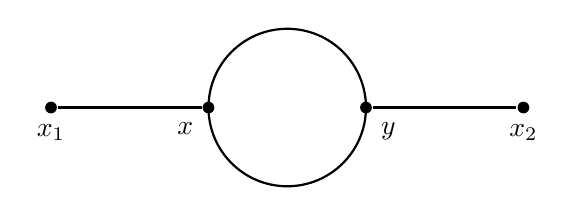
\begin{tikzpicture}[
                    thick,
                    dot/.style={circle, fill=black, inner sep=1.5pt}
                ]
                \draw (3,0) circle (1cm);

                \node[dot, label=below:$x_1$] (x1) at (0,0) {};
                \node[dot, label=below left:$x$]  (x)  at (2,0) {};
                \node[dot, label=below right:$y$] (y)  at (4,0) {};
                \node[dot, label=below:$x_2$] (x2) at (6,0) {};

                \draw (x1) -- (x);
                \draw (y)  -- (x2);

            \end{tikzpicture}
            \caption{Feynman diagram for the second order correction to the 2-point function in a \(\phi^3\) theory: each internal point corresponds to an interaction vertex, connected to three lines, each corresponding to a propagator.}
        \end{minipage}
        \hfill
        \begin{minipage}{0.5\textwidth}
            \begin{itemize}
                \item \(x_1, \, x_2\) external points, represented as dots.
                \item \(x, \, y\) internal points, represented as vertices.
                \item \(D_{x 1}\) and \(D_{y 2}\) propagators, represented as lines connecting the external points to the internal points.
                \item \(D_{x y}^2\) propagators, represented as two lines connecting the internal points \(x\) and \(y\).
            \end{itemize}
        \end{minipage}
    \end{figure}
\end{example}

More generally, we can write the \textbf{Feynman rules} for an n-point function as
\begin{itemize}
    \item N external points \(x_1, x_2, \ldots, x_n\), each connected to only one propagator (line) in every theory.
    \item Any number of vertexes, each corresponding to an interaction term in the Lagrangian
          \[
              i \int \mathrm{d}^4 z \, \mathcal{L}_{\text{int}} (z),
          \]
          where in particular for our \(\phi^3\) theory, we had
          \[
              i \int \mathrm{d}^4 z \, (-\frac{\lambda}{3!} \phi^3 (z)) = -i \frac{\lambda}{3!} \int \mathrm{d}^4 z \, \phi^3 (z),
          \]
          which means that each vertex has to be connected to three lines, since the interaction term is cubic in the field.
    \item Every vertex is of order \(O(\lambda)\), since it comes from the interaction Lagrangian, and thus the order of the correction is given by the number of vertexes in the diagram.
    \item The propagators as lines connects ALL the points, since the contractions has to be complete, since we cannot have uncontracted fields in the vacuum expectation value.
\end{itemize}
These rules telling us how to draw the Feynman diagrams for a given process, and they also allow us to write down the mathematical expression corresponding to each diagram without having to calculate all the contractions explicitly, which is a very powerful tool for calculating physical quantities in QFT.

The procedure of calculating a physical quantity using Feynman diagrams can be summarized as follows:
\begin{enumerate}
    \item Draw all the possible Feynman diagrams for the process you want to calculate, following the Feynman rules.
    \item For each vertex, we have an expression to write down the corresponding factor from the interaction Lagrangian \(\to  -i \alpha \int \mathrm{d}^4 z\).
    \item For each line, write down the corresponding Feynman propagator \(D_F (x,y)\).
\end{enumerate}

\subsubsection{Diagram Prefactors}

We have to understand how to put the correct prefactors \(\alpha\) in front of the integrals. Let us start from the interaction Lagrangian, which is given by
\[
    \mathcal{L}_{\text{int}} = \frac{\lambda^N}{N!} \phi^N,
\]
then a diagram with \(M\) vertexes (obtained considering corrections up to order \(O(\lambda^M)\)) and any number of external points will have
\begin{itemize}
    \item \(M!\) ways of permuting the vertexes, since they are indistinguishable.
    \item \(N!\) ways of permuting the fields in each vertex, since they are also indistinguishable, thus a total of \((N!)^M\) ways of permuting the fields in all the vertexes.
\end{itemize}
Putting all these factors together, we get a factor of \((N!)^M \times M!\) only from the counting of the permutations of the vertexes and fields, and thus we need to divide by this factor to avoid overcounting, since we are summing over all the possible contractions, which already takes into account all the possible permutations of the vertexes and fields.

An example of naive counting of the factors for a diagram with \(M\) vertexes and \(N\) fields in each vertex would give us a factor of
\[
    (N!)^M \times M! \times (\frac{\lambda}{N!})^M \times \frac{1}{M!},
\]
where the first factor comes from the permutations of fields in each vertex, the second factor comes from the permutations of the vertexes, the third factor comes from the interaction Lagrangian, and the last factor comes from the expansion of the exponential of the interaction Lagrangian. Is it possible that all these factors cancel out and we are left with a factor of \(\lambda^M\) for a diagram with \(M\) vertexes?

No, this counting is not correct, since we have to take into account that some diagrams may be equivalent under permutations of the vertexes and fields, and thus we need to divide by the number of symmetries of the diagram: \textit{the number of permutations of the vertexes and fields that leave the diagram unchanged}. This is known as the \textbf{symmetry factor} of the diagram, and it can be calculated by counting the number of ways to permute the vertexes and fields without changing the diagram.

Thus the correct factor for a diagram with \(M\) vertexes and \(N\) fields in each vertex is given by the inverse of the symmetry factor of the diagram, which can be calculated by counting the number of ways to permute the vertexes and fields without changing the diagram:
\begin{definition}[Symmetry factor]
    The symmetry factor of a Feynman diagram is the \textbf{number of independent transformations} (permutations of the vertexes and fields in the diagram) \textbf{mapping the diagram onto itself} (with external points fixed), and it is denoted by \(S\). The contribution of a diagram to a physical quantity is given by the inverse of the symmetry factor, which is \(1/S\). The \uline{identity has to be counted} as a symmetry, while \uline{swapping external points is not a symmetry}, since they are fixed. One can sum the symmetries of the drawing by hand, or one can multiply the symmetry prefactors of the subdiagrams (\(D_{xy}\), \(D_{xx}^2\)...).
\end{definition}

\begin{example}[Back to the cubic interaction]
    Let us go back to the second order correction to the 2-point function in the \(\phi^3\) theory, which corresponds to the following diagram:
    \begin{figure}[H]
        \begin{minipage}{0.45\textwidth}
            \centering
            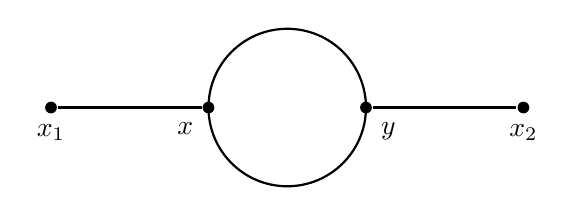
\begin{tikzpicture}[
                    thick,
                    dot/.style={circle, fill=black, inner sep=1.5pt}
                ]
                \draw (3,0) circle (1cm);

                \node[dot, label=below:$x_1$] (x1) at (0,0) {};
                \node[dot, label=below left:$x$]  (x)  at (2,0) {};
                \node[dot, label=below right:$y$] (y)  at (4,0) {};
                \node[dot, label=below:$x_2$] (x2) at (6,0) {};

                \draw (x1) -- (x);
                \draw (y)  -- (x2);

            \end{tikzpicture}
            \caption{Feynman diagram for the second order correction to the 2-point function in a \(\phi^3\) theory: each internal point corresponds to an interaction vertex, connected to three lines, each corresponding to a propagator.}
        \end{minipage}
        \hfill
        \begin{minipage}{0.5\textwidth}
            This diagram has two vertexes, each connected to three lines, and thus it corresponds to a correction of order \(O(\lambda^2)\). It can be obtained from 18 different contractions:
            \begin{itemize}
                \item 3 choices of \(\phi_x\) in \(\bcontraction[0.5ex]{}{\phi}{_1}{\phi} \phi_1 \phi_x\);
                \item 3 choices of \(\phi_y\) in \(\bcontraction[0.5ex]{}{\phi}{_2}{\phi} \phi_2 \phi_y\);
                \item 2 choices of the remaining \(\phi_y\) to be contracted with the first remaining \(\phi_x\).
            \end{itemize}
        \end{minipage}
    \end{figure}
    These 18 contractions have to be multiplied by 2 for the swap of the two vertexes \(x \leftrightarrow y\). Thus we get a total of 36 contractions which has to be divided by \((3!)^2 \times 2! = 72\), which is the number of permutations of the fields in the vertexes and the number of permutations of the vertexes, thus we get a symmetry factor of \(S=2\) for this diagram, and thus its contribution to the 2-point function is given by
    \[
        \frac{1}{2} \times (-i \frac{\lambda}{3!})^2 \int \mathrm{d}^4 z_1 \, \mathrm{d}^4 z_2 \, D_{x z_1} D_{y z_1} D_{z_1 z_2}^2,
    \]
    where the factor of \(1/2\) comes from the symmetry factor of the diagram, and the rest of the factors come from the interaction Lagrangian and the Feynman propagators.

    In order to understand the symmetry factor of this diagram, we can also look at it from a different perspective; if we rewrite the contraction, we can see that permuting the propagators between the internal points \(x\) and \(y\) does not change the diagram, since they are indistinguishable:
    \[
        \bcontraction[0.5ex]{}{\phi_1}{\phi_2}{\phi_x}
        \bcontraction[1ex]{\phi_1}{\phi_2}{\phi_x\phi_x\phi_x}{\phi_y}
        \contraction[0.5ex]{\phi_1\phi_2\phi_x}{\phi_x}{\phi_x\phi_y}{\phi_y}
        \contraction[1ex]{\phi_1\phi_2\phi_x\phi_x}{\phi_x}{\phi_y\phi_y}{\phi_y}
        \phi_1 \phi_2 \phi_x \phi_x \phi_x \phi_y \phi_y \phi_y
        \quad = \quad
        \bcontraction[0.5ex]{}{\phi_1}{\phi_2}{\phi_x}
        \bcontraction[1ex]{\phi_1}{\phi_2}{\phi_x\phi_x\phi_x}{\phi_y}
        \contraction[1ex]{\phi_1\phi_2\phi_x}{\phi_x}{\phi_x\phi_y\phi_y}{\phi_y}
        \contraction[0.5ex]{\phi_1\phi_2\phi_x\phi_x}{\phi_x}{\phi_y}{\phi_y}
        \phi_1 \phi_2 \phi_x \phi_x \phi_x \phi_y \phi_y \phi_y,
    \]
    and if we compare it to the graphical representation of the diagram, we can see that this contraction symmetry corresponds to the invariance of the diagram under the \textbf{vertical flip symmetry}, which is a symmetry of the diagram that leaves the external points fixed and swaps the internal points \(x\) and \(y\). This symmetry is the only non-trivial symmetry of the diagram and thus we have a total of 2 symmetries (do not forget the identity), which gives us a symmetry factor of \(S=2\), and thus a contribution of \(1/2\) for this diagram.
\end{example}

It can even happen to have an internal subdiagram that is disconnected from the external points, which is called a \textit{vacuum bubble}, and it is possible to show that the contribution of a vacuum bubble cancels out with the denominator of the Green's function. For example, if we were to compute the next order corrections to the 2-point function, we would get the following diagrams:
\[
    \begin{aligned}
        \bra{\Omega} \hat{T} \{ \hat{\phi} (x) \hat{\phi} (y) \} \ket{\Omega} \Big|_{\text{num}}
         & = \quad \feynTree                                                                                  \\[2pt]
         & + \quad \feynBubble \quad + \quad \feynDoubleTadpole \quad + \quad \feynCactus                     \\[2pt]
         & + \quad \feynDiscDoubleTadpole \quad + \quad \feynDiscSunset \quad + \quad \mathcal{O}(\lambda^4),
    \end{aligned}
\]
where the fifth and sixth diagrams have vacuum bubble. The complete expression associated to these diagrams is given by
\[
    \begin{aligned}
        \bra{\Omega} \hat{T} \{ \hat{\phi} (x) \hat{\phi} (y) \} \ket{\Omega} \Big|_{\text{num}} & = D_{12} + (-i \lambda)^2 \int \mathrm{d}^4 x \,\mathrm{d}^4 y \, \left( \tfrac{1}{2} D_{1x} D_{2y} D_{x y}^2 + \tfrac{1}{4} D_{1x} D_{xx}^2 D_{2y} D_{yy}^2\right. \\
                                                                                                 & + \left. \tfrac{1}{2} D_{1x} D_{2x} D_{xy} D_{yy} + D_{12} (\tfrac{1}{8} D_{xx} D_{xy} D_{yy} + \tfrac{1}{12} D_{xy}^3) \right) + \mathcal{O}(\lambda^4),
    \end{aligned}
\]
where the contribution of the vacuum bubbles can be canceled out with the denominator of the Green's function, which is given by
\[
    \bra{\Omega} \hat{T} \{ \hat{\phi} (x) \hat{\phi} (y) \} \ket{\Omega} \Big|_{\text{den}} = \frac{1}{\bra{0} \hat{T} \{ \exp[ i \int \mathrm{d}^4 z \, \mathcal{L}_{int} ] \} \ket{0}}.
\]
Thus the denominator is exactly a Green's function with no external points, and thus it contains only \textbf{vacuum diagrams}, which are disconnected from the external points, and thus they do not contribute to the physical quantity we are calculating, and thus they can be canceled out with the denominator. This is a very important result, as it tells us that we can ignore the vacuum bubbles when calculating physical quantities in QFT: they do not contribute to the final result, and thus we can focus only on the connected diagrams, which are the ones that contribute to the physical quantity we are calculating. Indeed we have:
\begin{itemize}
    \item Numerator: \(\left(\sum \text{connected diagrams}\right)\left(1 + \sum \text{vacuum diagrams} \right)\).
    \item Denominator: \(\left(1 + \sum \text{vacuum diagrams}\right)\).
\end{itemize}
Thus in the end, the contribution of the vacuum diagrams cancels out, and we are left with only the connected diagrams, which are the ones that contribute to the physical quantity we are calculating:
\[
    \bra{\Omega} \hat{T} \{ \hat{\phi} (x) \hat{\phi} (y) \cdots \hat{\phi} (z) \} \ket{\Omega} = \sum \text{connected diagrams}.
\]

\begin{example}[Still on the cubic interaction]
    If we were to show the previous result explicitly for the \(\phi^3\) theory, we would have to compute the green's function up to order \(O(\lambda^4)\), which would give us the following diagrams:
    \[
        \begin{gathered}
            \bra{\Omega} \hat{T} \{ \hat{\phi} (x) \hat{\phi} (y) \} \ket{\Omega}                                                                                                                                                                                                                                                                                                     \\
            = \frac{\left( \scalefeyn{0.7}{\feynTree} + \scalefeyn{0.7}{\feynBubble} + \scalefeyn{0.7}{\feynDoubleTadpole} + \scalefeyn{0.7}{\feynCactus} \right)\left(1 + \scalefeyn{0.7}{\feynDiscDoubleTadpole} + \scalefeyn{0.7}{\feynDiscSunset} \right)}{\left(1 + \scalefeyn{0.7}{\feynDiscDoubleTadpole} + \scalefeyn{0.7}{\feynDiscSunset} \right)} + \mathcal{O}(\lambda^4) \\
            = \scalefeyn{0.7}{\feynTree} + \scalefeyn{0.7}{\feynBubble} + \scalefeyn{0.7}{\feynDoubleTadpole} + \scalefeyn{0.7}{\feynCactus} + \mathcal{O}(\lambda^4),
        \end{gathered}
    \]
    which shows explicitly that the contribution of the vacuum bubbles cancels out with the denominator, and thus we are left with only the connected diagrams, which are the ones that contribute to the physical quantity we are calculating.
\end{example}

\subsubsection{Summary of Feynman Rules in Position Space}

Let us group and summarize all the Feynman rules we have derived so far for a scalar field theory in position space:

\begin{itemize}
    \item \textbf{External point}: \(x_i\), represented as a dot, and it is connected to only one propagator.
    \item \textbf{Vertex}: \(i \int \mathrm{d}^4 z \, \mathcal{L}_{\text{int}} (z)\), represented as a dot and connected to a number of lines equal to the number of fields in the interaction term. It is specific to the theory we are considering, since it depends on the interaction Lagrangian, and thus it can be different for different theories.
    \item \textbf{Propagator}: \(D_F (x,y)\), represented as a line connecting two points, and corresponding to the Feynman free propagator between those two points.
    \item \textbf{Symmetry factor}: \(1/S\), where \(S\) is the number of symmetries of the diagram, which can be calculated by counting the number of ways to permute the vertexes and fields without changing the diagram. It contains the identity as a symmetry, while swapping external points is not a symmetry, since they are fixed.
    \item \(\bra{\Omega} \hat{T} \{ \hat{\phi} (x) \hat{\phi} (y) \cdots \hat{\phi} (z) \} \ket{\Omega} = \sum \text{connected diagrams}\), since the contribution of the vacuum diagrams cancels out with the denominator of the Green's function, and we can focus only on the connected diagrams, which are the ones contributing to the physical quantity we are calculating.
\end{itemize}
